\section{Introduction of the ExtraSensory Dataset}

The ExtraSensory dataset was collected in 2015 and 2016 by Yonatan Vaizman and Katherine Ellis under the supervision of Professor Gert Lanckriet. It is based on sensor data from smartphones and smartwatches produced by 60 participants in intervals of one minute. In contrast to many other datasets, the data was generated by normal everyday devices using multiple sensors at the same time. Furthermore, the participants behavior was not scripted like in many other case studies and they were allowed to behave in an natural way. The sensors included an accelerometer, gyroscope, location and audio sensor. Almost every participant used practically every sensor in the activity recordings. Additionally some participants used smart watches or fitness tracker which provided the additional watch accelerometer.

The users themselves assigned most of their data points to the respective activities. In the course of this they had the option to use predefined labels or create their own. The label represented various information about the location, the context and the activity of a user. Some examples are 'in class', 'singing', 'stairs (going up)', 'stairs (going down)', 'with friends' or 'talking'. In a preprocessing step these label were reduced to a set of 51 labels by combining similar labels. 

The final results contained 377,346 data points, which were described with one or more of the 51 final labels. 

\begin{figure}[H]
	\begin{center}
		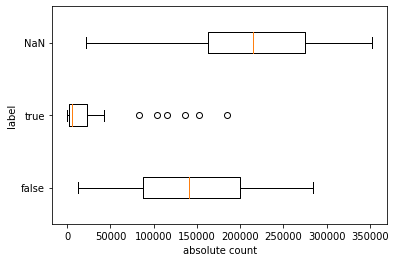
\includegraphics[scale=.8]{images/boxplot_label.png}
		\caption{A box-plot showing the distribution of the absolute count of a given value (false, true or NaN) over the different labels. The yellow line represents the median, the rectangle the 25\% percentile, the line the 75\% percentile and the dotes are outliers.}
		\label{abb:boxplot_label}
	\end{center}		
\end{figure}

\newpage
This means that for each data point a label vector of length 51 exists. Each entry can contain the values 'true', 'false' or 'NaN', where 'NaN' represents missing information on this label.

Figure \ref{abb:boxplot_label} visualizes the distribution of these values for each label as a box-plot diagram. Looking at the median for 'NaN', it can be seen that for most labels the majority of data points do not contain a value - which increases the difficulty of classification. This means that for many labels there exists a large number of data points in the ExtraSensory data set that do not contain any information regarding the label.

Furthermore, it can be seen that the median of labels with the value 'true' is just 5,153 meaning that in the median only 5,153 samples exist for a specific activity. Overall only very few labels at all are labeled as 'true' for more than 10\% of the data points, consequently there are many label classes consisting of very few representatives. 

\begin{figure}[h]
	\begin{center}
		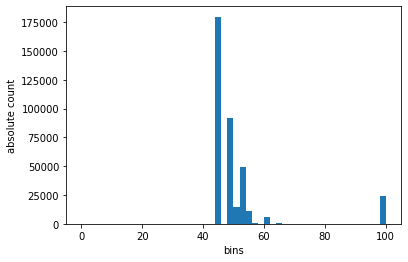
\includegraphics[scale=.8]{images/hist.png}
		\caption{Histogram of absolute counts of percentage of NaN values for each data point. The data is distributed into 50 bins. Each bin has the size of 2 \% of the labels.}
		\label{abb:histogramm_data}
	\end{center}		
\end{figure}

Finally, it can be seen that in all data points at least 44\% of the 51 labels are not evaluated. Thus, there are no data points that make statements about all labels at the same time, the data therefore is sparse in a variety of ways.